\vspace{-0.2in}

\section{State Space Analysis}
\label{sec:State_Space_Analysis}

%\vspace{-0.4in}

\begin{figure}[t]
	\centering
	\begin{subfigure}[b]{0.5\textwidth}
		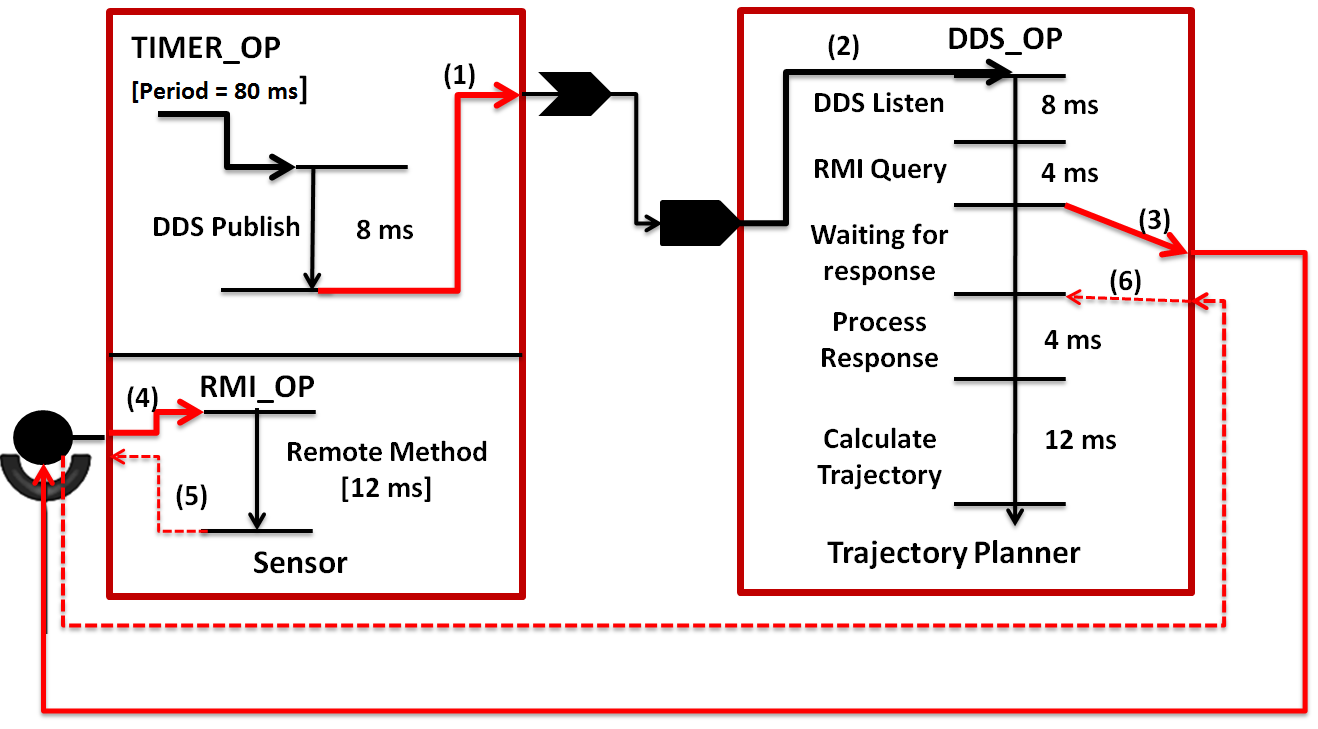
\includegraphics[width=\textwidth]{./figs/tpa}
		\caption{Component Assembly}
		\label{fig:tpa}
	\end{subfigure}%
	\begin{subfigure}[b]{0.5\textwidth}
		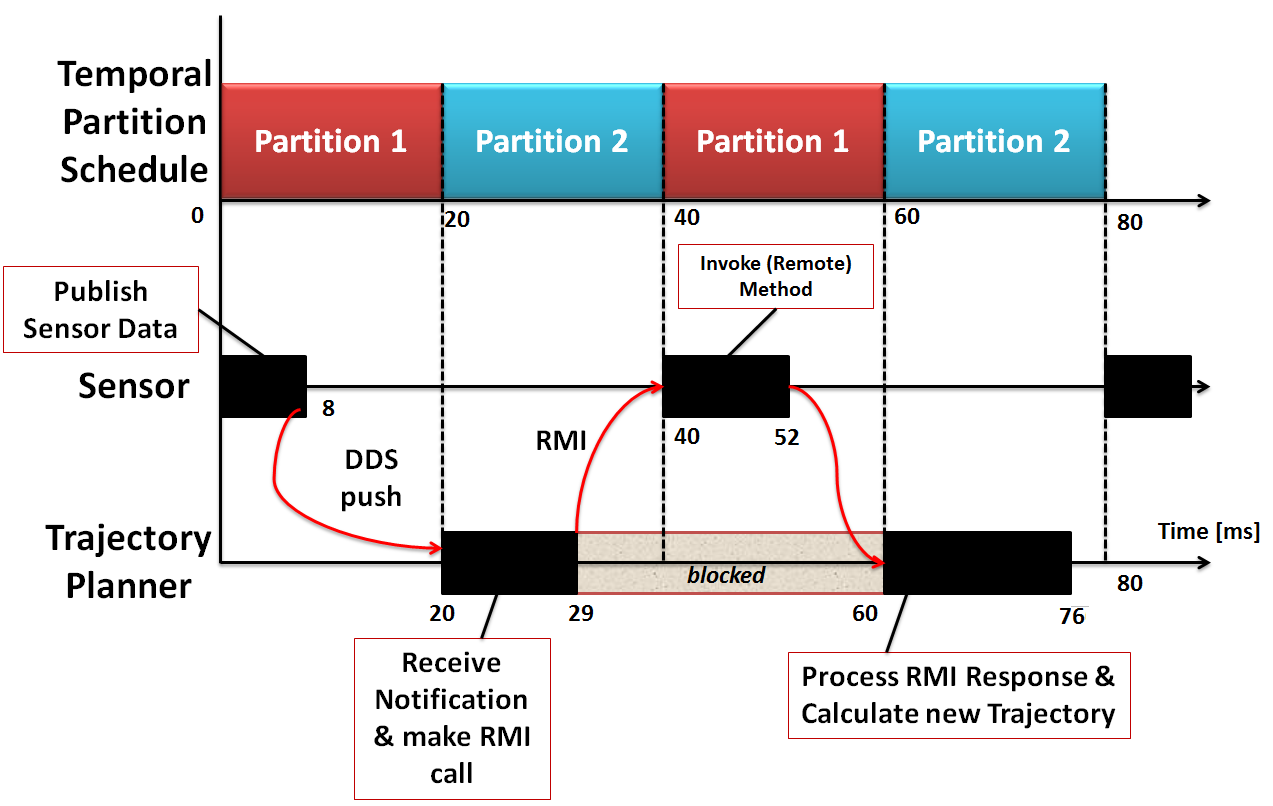
\includegraphics[width=\textwidth]{./figs/tpa_td}
		\caption{Timing Diagram}
		\label{fig:tpa_td}
	\end{subfigure}
	\caption{Trajectory Planning Application}\label{fig:TPA}
%\vspace{-0.2in}
\end{figure}



Given a CPN model (that was generated from a component architecture and deployment model), a state-space of the system can be constructed using the semantics of CPN. This state space is infinite, however, in practice, it is often sufficient to consider some finite subset, starting from a initial state up to a few hyperperiods of the partition scheduler. In order to describe the utility of state space analysis, we consider a simple trajectory planning application (TPA). The component assembly for this application is shown in Figure \ref{fig:tpa}. A Sensor component periodically publishes on a trigger topic, notifying the Trajectory Planner of the existence of new sensor data. Once the notification is received, the Trajectory Planner makes an RMI call to retrieve the data structure of sensor values, using which the satellite trajectory is updated. The sequence of steps in each of these operations is referred to as the business logic of the operation. This business logic is modeled using a textual language in the modeling tools, in which the designer specifies the macro execution steps in a component operation along with worst-case estimated time taken on each step. Figure \ref{fig:tpa_td} shows the expected timing diagram. 

The analyzable states of this system are observed in the markings of the various CPN places in the model. Using the built-in state space analysis in \textit{CPN Tools} a bounded state space of the system is generated. Using both standard and user-defined queries, this state space is searched to check system properties like lack deadline violations and deadlocks, bounds on response times etc.

\vspace{-0.1in}

\subsubsection{Deadline Violation Detection:}

Each time a component operation is scheduled, the clock value of the node is recorded as the "start time" of the operation. If this operation is incomplete when the clock reaches the operation's deadline, a deadline violation is detected. Using the \emph{SearchNodes} function in CPN Tools, the deadline violations on any component operation can be identified by observing all component operations each time the node-specific clock progresses. In Figure \ref{fig:tpa_td}, the \emph{DDS\_OP} on the Trajectory Planner takes 56 ms to complete, measured from when the operation was enqueued and marked as ready. If the deadline of this operation is set to 50 ms, a state space search would reveal a deadline violation when the clock reaches 51 ms.

\vspace{-0.1in}

\subsubsection{Worst-case Trigger-to-Response Time Calculation:}

For a known trigger operation and desired response operation, the worst-case trigger-to-response time can also be calculated from the generated state space. Using the names of the trigger and response operations, a state space node that presents the earliest completion of the trigger operation and the latest completion of the response operation within the set period is identified. In the Trajectory Planning application, considering the \emph{TIMER\_OP} to be the trigger and the trajectory planning \emph{DDS\_OP} to be the response, the worst-case response time is found to be 68 ms (Trigger completes earliest at 8 ms and response completes latest at 76 ms). 

\vspace{-0.1in}

\subsubsection{Partial Thread Execution Order Generation:}

In development scenarios where an application developer is aware of the operation-specific timing requirements but not thread priorities, the analysis is capable of identifying partial thread execution orders that satisfy the requirements. If all unknown thread priorities are set to a common value, the generated partial state space will then encapsulate the set of non-deterministic thread execution orders that arise from the scheduling. Using timing requirements of the form - \emph{Once Operation A on Component A on Node A completes, Operation B on Component B on Node B must complete within 150 ms}, a state space node satisfying this requirement can be identified by querying the generated state space. A backtrace from this node enables assigning thread priorities to ensure the satisfaction of the timing requirement.

\vspace{-0.15in}
\subsubsection{Scalability Testing:}
\label{sec:Scalability_Testing}

The size of the generated state space is dependent on the amount of concurrency in the behavior. If all the executing threads had unique priorities, the thread execution order is a constant as the scheduling is priority-based. However, for large systems with groups of applications and increased concurrency, an equally large state space is required to observe the tree of possible thread executions and operational behaviors. This analysis model has been identified to scale well for medium-sized applications, tested up to 100 components distributed on up to 5 computing nodes. Table \ref{table:scalability} summarizes these results.

\vspace{-0.1in}

\section{Analysis Model Generation}
\label{sec:Model_Generation}

\vspace{-0.1in}

As mentioned in Section \ref{sec:CPN_Modeling}, the control flow and timing details of component operations are directly integrated into the design-time modeling framework. Using the formal domain-specific model of the system, the configuration of the partition scheduling and component assembly are derived and translated into meaningful CPN tokens. The business logic of each component operation is expressed using a textual language with one attribute per interaction per instance of each component being deployed. Model interpreters parse through this complete design model, instantiating CPN model templates and combining these instances to generate a single integrated .cpn file to analyze the entire system.

%\vspace{-0.4in}

\begin{table}[t]
	\caption{Scalability Results}
	\label{table:scalability}
	\begin{center}
		\begin{tabular}{ | c | p{1cm} | p{1.7cm} | p{1.7cm} | p{1.4cm} | p{1.3cm} | p{1.7cm} |}
			\hline
			Scenario & Nodes & Partitions / Node & Threads / \mbox{Partition} & Hyper-periods & State Space & Generation Time\\ \hline
			TPA & \multicolumn{1}{|c|}{5} & \multicolumn{1}{|c|}{2} & \multicolumn{1}{|c|}{1} & \multicolumn{1}{|c|}{10} & \multicolumn{1}{|c|}{180} & \multicolumn{1}{|c|}{0.981s}\\ \hline
			Sample2 & \multicolumn{1}{|c|}{2} & \multicolumn{1}{|c|}{5} & \multicolumn{1}{|c|}{5} & \multicolumn{1}{|c|}{10} & \multicolumn{1}{|c|}{124,469} & \multicolumn{1}{|c|}{14.1m} \\ \hline
			Sample3 & \multicolumn{1}{|c|}{5} & \multicolumn{1}{|c|}{5} & \multicolumn{1}{|c|}{4} & \multicolumn{1}{|c|}{10} & \multicolumn{1}{|c|}{485,552} & \multicolumn{1}{|c|}{36.5m} \\ \hline			
		\end{tabular}
	\end{center}
\vspace{-0.2in}
\end{table}

%\vspace{-0.4in}
